% ============================================================================ CONVERTER + DSE
\section{Converter Synthesis and Design-Space Exploration}\label{sec:dse}

\subsection{Generalized hybrid regulator family}
The regulator is synthesized from a family rather than fixed in advance. The family is the
two-phase hybrid switched-capacitor--buck converter with $N$ switched-capacitor branches ($N$
high-side switches and $N-1$ flying capacitors) and $K$ inductor branches ($K$ low-side switches),
$K_A$ of them driven in the first phase, and the branch-allocation vector $\mathbf{B}$ with
$\sum_i B_i = N$; the duty ratio is $D = NV_{\mathrm{out}}/V_{\mathrm{in}}$~\cite{Abdelzaher2025ECTC,
Abdelzaher2026EPEPS}. The double series-capacitor buck and the dual-phase multi-inductor hybrid
are members~\cite{DSCH,DPMIH44}. A closed-form continuous-conduction loss model evaluates
conduction in the switches with the inductor ripple, the flying-capacitor equivalent series
resistance and the inductor winding resistance, together with high-side overlap, gate-drive and
output-capacitance switching loss. Against circuit simulation of four published
members---$N/K = 2/2$, $3/2$, $4/4$ and $6/2$ at 48-to-1~V, 30~A and 500~kHz with common
components---the model reproduces total loss to $94.4\pm1.5$\,\% (worst case
92.9\,\%)~\cite{Abdelzaher2025ECTC}, and the extended framework to
$95.3\pm1$\,\%~\cite{Abdelzaher2026EPEPS}. Inductor core loss, alternating-current winding
resistance, dielectric loss and dead-time loss are not in the model; Section~\ref{sec:explore}
bounds them for every compared case and every regulator count.

\subsection{Synthesis}
For a specification---output current and voltage, input voltage, a target current density
$J_{\mathrm{t}}$ and ripple limits---the synthesis enumerates every member with at most 15
components ($2N + 2K - 1 \le 15$, $2\le K\le N$), with $K_A = \lceil K/2\rceil$ and $\mathbf{B}$
the balanced allocation of the branches to the two phases~\cite{Abdelzaher2026EPEPS}. For each
member it searches exhaustively over the library parts that pass the hard constraints---every
combination of high-side device, low-side device, inductor, capacitor and switching frequency on a
50-point logarithmic grid from 43~kHz to 200~MHz, up to the inductor's rated frequency---and
returns the combination of lowest loss at 25\,$^\circ$C. The library holds 90 enhancement-mode GaN
transistors, 11 integrated inductors and 8 capacitors. The hard constraints are the device
voltage rating ($\ge V_{\mathrm{in}}/N$ high side, $\ge V_{\mathrm{out}}$ low side), the 5-V gate
rating and the continuous current rating ($\ge I_{\mathrm{out}}/N$ high side,
$\ge \max(\mathbf{B})I_{\mathrm{out}}/N$ low side); the inductor saturation current
($\ge \max(\mathbf{B})I_{\mathrm{out}}/N$) and rated frequency; the capacitor voltage rating;
the inductor ripple ($|\Delta I| < 0.5\,I_{\mathrm{out}}$) and the output ripple
($\Delta V_{\mathrm{out}} < 0.25\,V_{\mathrm{out}}$ with 50~\textmu F per cell); and the area
budget, which compares the largest tier footprint of the stacked cell,
$\max(NA_{\mathrm{HS}}, KA_{\mathrm{LS}}, KA_{L}, (N-1)A_{C})$, with $I_{\mathrm{out}}/J_{\mathrm{t}}$.
$J_{\mathrm{t}}$ is thus a minimum current density: the selected cell occupies 5.61~mm$^2$ of its
\DseFortyNineBudget-mm$^2$ budget, \DseFortyNineJ~A\,mm$^{-2}$. Temperature, manufacturability
and mechanical response are not constraints of the synthesis; they are evaluated afterward on
the package. One synthesis takes 4.6~s on one core. Device on-resistance is scaled with
temperature by the typical normalized curves of the selected parts, $6.0\times10^{-3}$\,K$^{-1}$
for the high-side EPC2014C and $8.0\times10^{-3}$\,K$^{-1}$ for the low-side EPC2057 over
25--125\,$^\circ$C~\cite{EPC2014C_DS2021,EPC2057_DS2025}, and each device is evaluated at the
in-cell temperature of its own tier.
\emph{Capacitor rule (corrected).} In this family the flying capacitor $C_i$ holds
$(N-i)V_{\mathrm{in}}/N$---32 and 16~V for $C_1$ and $C_2$ of the selected cell---while every
switch blocks $V_{\mathrm{in}}/N$. The published synthesis compared every capacitor with
$V_{\mathrm{in}}/N$, which admitted a 25-V part for the 32-V $C_1$. The rule now requires each
flying capacitor's derated rating (80\,\%) to cover its own stress and its effective capacitance
under bias, temperature and tolerance to hold the switching ripple below 10\,\% of its voltage; the
equivalent series resistance is taken at the switching frequency where the vendor publishes it.
Because the flying capacitors are soft-charged through the inductors, only that resistance enters
the loss. Under the corrected rule the 49-cell synthesis returns the same topology, devices and
frequency with a rated 0603 100-V X7T capacitor, 0.27~\textmu F at 32~V and 7.8~m$\Omega$ at
805~kHz (Table~\ref{tab:spec}), which raises the cell loss by 0.06~W; the published rule is kept
as a reproducible legacy configuration.

\begin{figure}[!t]
\centering
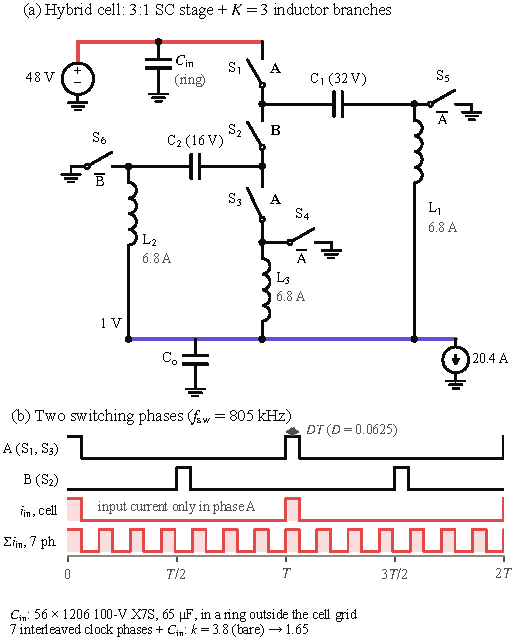
\includegraphics[width=\columnwidth]{fig2_converter.pdf}
\caption{(a) The synthesized cell, $N{=}3$, $K{=}3$, $K_A{=}2$: a 3:1 switched-capacitor stage
(S$_1$--S$_3$; $C_1$ at 32~V, $C_2$ at 16~V) feeding three inductor branches of
$I_{\mathrm{cell}}/3 = 6.8$~A. (b) S$_1$ and S$_3$ conduct in phase A and drive $L_1$ and
$L_3$ at 16~V; S$_2$ conducts in phase B and drives $L_2$; S$_4$--S$_6$ freewheel the undriven
inductors ($D = 0.0625$, $f_{\mathrm{sw}} = 805$~kHz). The 48-V input current flows only in
phase A; $C_{\mathrm{in}}$ is the package input capacitance (56 1206 100-V X7S capacitors,
65~\textmu F at 48~V) in a ring outside the cell grid, and the clocks of the 49 cells are interleaved
in seven phases, which together hold the RMS-to-average ratio of the package input current at
$k = \DecapKeq$ (bare pulse: \DecapKopen; Section~\ref{sec:evaluate}).}
\label{fig:converter}
\end{figure}

\subsection{Regulator count and architecture}
The design-space mode repeats the synthesis over the regulator count $M$ and scores every
candidate with its conversion loss and the system-level routing model of the vertical
interconnect chain and the lateral redistribution path of~\cite{Krishnakumar2026DVPD}, at
25\,$^\circ$C. It is an electrical screen: the strongest candidates are then carried through the
coupled chain (Section~\ref{sec:explore}). Fig.~\ref{fig:dse} shows the screen for a 1-kW,
48-to-1-V load on a 500-mm$^2$ die at $J_{\mathrm{t}} = 3.5$~A\,mm$^{-2}$ over the
\DseNcounts{} counts sampled (\DseCounts). When the topology is re-synthesized at every count,
the selected member changes three times---$N/K = 4/4$, $2/2$, $3/3$ and again $2/2$---and each
jump in Fig.~\ref{fig:dse} is a constraint becoming active: at $M = 40$ the four-branch tier
(7.20~mm$^2$) no longer fits the 7.14-mm$^2$ budget, and at $M = 56$ the smallest three-branch
tier (5.40~mm$^2$) no longer fits 5.10~mm$^2$. Within a member the loss falls with the cell current
and steps when a device, the capacitor or the frequency changes (Table~S2). The minimum lies at
$M = \DseCorrOptM$ ($N2K2K_A1$ at \DseOptFsw~kHz, \DseCorrOptLoss~W under the corrected capacitor rule,
\DseOptLoss~W with the published one), the $3/3$ family reaches its best
at $M = \DseThreeBestM$ (\DseThreeBestLoss~W), and from $M = \DseFirstInfeasibleM$ the budget
(\DseFirstInfeasibleBudget~mm$^2$) is smaller than the smallest two-branch device set that meets
the current rating (3.74~mm$^2$), so no member is feasible. Holding the topology fixed instead
truncates the feasible range at $M = 52$. The seventeen counts take about four minutes on one
core. At $M = 49$ the screen gives \DseFortyNineLoss~W (\DseFortyNineConv~W conversion,
\DseFortyNineRoute~W routing); the package ledger of Section~\ref{sec:models} returns \PIsoZone~W
at 25\,$^\circ$C for the embedded integration---the same conversion loss and a smaller routing
loss from the explicit package conductors---so the two differ only in the routing model.

\begin{figure}[!t]
\centering
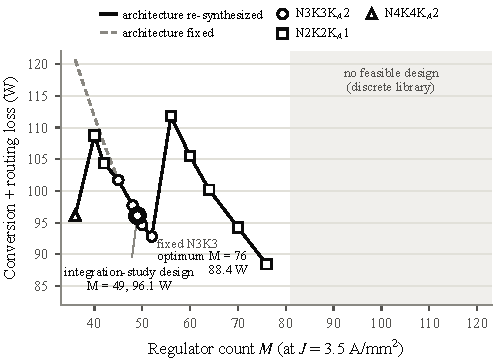
\includegraphics[width=\columnwidth]{fig_dse.pdf}
\caption{(a) Electrical screen of the regulator count: conversion plus system-level routing loss
at 25\,$^\circ$C against $M$ at $J_{\mathrm{t}} = 3.5$~A\,mm$^{-2}$ with the discrete library, topology
re-synthesized at every count under the corrected flying-capacitor rule (solid; markers at the
\DseNcounts{} sampled counts) and the published rule (faded), and held at $N3K3K_A2$ (dashed). Jumps
mark an active area or rating constraint; no member is feasible from $M = \DseFirstInfeasibleM$; the
integration design point is ringed. (b) Package-internal loss of the 49-cell design and of the 64-cell
candidate through the full coupled chain (Z1, cooling~A), a different boundary from the screen.}
\label{fig:dse}
\end{figure}

The integration study of Sections~\ref{sec:evaluate}--\ref{sec:explore} uses one design point
for every architecture, so that any difference between the architectures is caused by the
integration and not by the regulator: $M = 49$ cells on a $7\times7$ grid at
$J_{\mathrm{t}} = 3.5$~A\,mm$^{-2}$, the areal utilization of the reference
framework~\cite{Krishnakumar2026DVPD} and the largest square grid near the electrical screen's
plateau. At that count the search returns the regulator of Table~\ref{tab:spec}---$N3K3K_A2$ with
EPC2014C and EPC2057 devices at 805~kHz, 1.87~W per cell at 25\,$^\circ$C---so the regulator
carried into the package is the synthesis output, not an assumption. Every switch blocks
$V_{\mathrm{in}}/N = 16$~V, 40\,\% and 32\,\% of the high- and low-side ratings; each inductor
carries 6.8~A with 4.7~A of peak-to-peak ripple, a 9.1-A peak against its 23-A saturation current;
the summed cell ripple is 9.0~A (44\,\% of the limit's 50\,\%) and the output ripple 28~mV.

\begin{table}[!t]
\caption{System specification, synthesized design point with ratings and operating stress, and
package and cooling parameters (full material and geometry data: Tables~S1--S4).}
\label{tab:spec}
\centering
\footnotesize
\setlength{\tabcolsep}{2pt}
\begin{tabular}{@{}lL{3.65cm}c@{}}
\toprule
Quantity & Value & Source \\
\midrule
\multicolumn{3}{@{}l}{\emph{Specification (inputs)}}\\
Load / platform rail & 1~kW at 1~V / 48~V & spec. \\
Compute die & $22.36\times22.36$~mm, 1~kW uniform & spec. \\
Regulator count, grid & 49, $7\times7$ & input \\
Target current density $J_{\mathrm{t}}$ & 3.5~A\,mm$^{-2}$, minimum: cell area $\le I_{\mathrm{cell}}/J_{\mathrm{t}}$ & input \\
Ripple limits & $\Delta I < 0.5\,I_{\mathrm{cell}}$; $\Delta V_{\mathrm{out}} < 0.25$~V & input \\
\midrule
\multicolumn{3}{@{}l}{\emph{Synthesized regulator (outputs; rating / operating stress)}}\\
Architecture $N/K/K_A$ & $3/3/2$, $\mathbf{B} = [1,1,1]$, $D = 0.0625$, 805~kHz & synthesis \\
High-side device & EPC2014C: 40~V / 16~V, 10~A, $T_J\le150\,^\circ$C, 16~m$\Omega$ & synthesis \\
Low-side device & EPC2057: 50~V / 16~V, 9.6~A, $T_J\le150\,^\circ$C, 8.5~m$\Omega$ & synthesis \\
Inductor ($\times3$) & 250~nH, 1.6~m$\Omega$, $I_{\mathrm{sat}}$ 23~A / 9.1~A peak, 500~\textmu m, shared-core interposer type~\cite{Rasheedi2026CoupledInductor} & synthesis \\
Flying capacitors $C_1$, $C_2$ & 32~V / 16~V stress. A1: 0603 1~\textmu F 100~V X7T (GRM188D72A105KE01), 0.27/0.59~\textmu F at 32/16~V, 7.8~m$\Omega$, 1.0~mm max; A0: 100-\textmu m tier, no qualifying part & synthesis \\
Output capacitance & 50~\textmu F per cell, in the inductor tier & synthesis \\
Input decoupling & 56 $\times$ 1206 4.7-\textmu F 100-V X7S in a ring outside the grid (65~\textmu F at 48~V); 7 interleaved clock phases; $k = \DecapKeq$ & design \\
Cell footprint & 5.61~mm$^2$ (2.37~mm square), 3.64~A\,mm$^{-2}$ & synthesis \\
Loss per cell at 25\,$^\circ$C & 1.87~W (1.67~W conduction) & synthesis \\
\midrule
\multicolumn{3}{@{}l}{\emph{Package and cooling}}\\
Power substrate & Si, 300~\textmu m, $30\times30$~mm; TSVs 30~\textmu m at 60~\textmu m & \cite{Krishnakumar2026DVPD} \\
Ball-grid array & 0.8~mm pitch, 0.4~mm SAC305 balls & \cite{Krishnakumar2026DVPD} \\
Board & IT-968G, 2.4~mm, homogenized Cu planes & arch. \\
Cold plate (each) & Si microchannels, water at 25\,$^\circ$C, 27~g\,s$^{-1}$, $\Delta p$ \CoolDp~kPa, \CoolPhyd~W hydraulic & design \\
Thermal interface & 50~\textmu m, 3~W\,m$^{-1}$K$^{-1}$ & design \\
\bottomrule
\end{tabular}
\end{table}
